\chapter{ОБЗОР ЛИТЕРАТУРЫ}\label{chap1}

%Первая глава всегда посвящена обзору литературы. В начале каждой главы необходимо написать небольшую аннотацию о содержании главы (так называемая \textit{врезка}). Например:

В настоящей глава формулируются основные понятия и определения,используемые в курсовой работе.Приводится классификация (согласно работе \cite{GabasovKirillovaPU}) принципов управления, используемых в современной теории управления,а так же их программные и позиционные решения.Объясняется принцип управления в режиме реального времени в применении к реализации оптимальных обратных связей в задачах оптимального управления с конечным горизонтом планирования \cite{GabasovDmitrukKirillova15a}.


%%%%%%%%%%%%%%%%%%%%%%%%%%%%%%%%%%%%%%%%%%%%%%%%%%%%%%%%%%%%%%%%%%%%%%%%%%%%%%%%
\section{Задачи оптимального управления}\label{1sec:optimal-control}
Человек занимается управлением на протяжении всей своей жизни для обеспечения желаемого течения тех или иных процессов или сам предпринимает необходимые действия и принимает соответсвующие решения.

Теория оптимального управления,отражающая современный этап развития вариационного исчелсения,возникла в середине \RNumb{20} века в связи с задачами, поставленными практикой в различных областях развития новой техники.

Существует два взгляда на теорию оптимального управления.Согласно одному из них,теория оптимального управления — раздел современного вариационного исчисления.В соотсветсвии с этим случаем введём следующее определние.
\begin{definition} Управления — элементы функциональных пространств, по которым ищется экстремум выбранного функционала качества.
\end{definition}
Главной задачей данной теории является анализ решения экстремальной задачи(существование, единственность, непрерывная зависимость решений, необходимые и достаточные условия оптимальности).

Другой взгяд трактует данную теорию как раздел современной теории управления, представляющей естественное развитие классической теории управления.
В этом случае выделим следующее определения для управления.
\begin{definition} Управления — это процесс, в котором для достижения нужного поведения объекта управления в каждый текущий момент времени создаются целенаправленные(управляющие) воздействия на объект управления в зависимотси от доступной к этому моменту информации о поведении объекта и действующих на него возмущений.
\end{definition}

%%%%%%%%%%%%%%%%%%%%%%%%%%%%%%%%%%%%%%%%%%%%%%%%%%%%%%%%%%%%%%%%%%%%%%%%%%%%%%%%
\section{Программные и позиционные решения}\label{1sec:Solution}

При управлении динамическим объектом используются три принципа: управление по разомкнутому контуру(программное управление), управление по замкнутому контуру(позиционное управление), управление в реальном времени.
\begin{definition} 
Программное управление — управление, при котором (программные) управляющие воздействия (программы) планируются по априорной информации до начала процесса управления и не корректируются в процессе управления. 
\end{definition}
\begin{definition} 
Позиционное управление — управление, при котором (позиционные) управляющие воздействия создаются в процессе управления по текущим позициям, которые аккумулируют информацию, доступную к текущему моменту.
\end{definition}
\begin{definition} 
Cинтез оптимальных систем управление — построение отпимальных позиционных управляющих воздействий.
\end{definition}
При создании систем по принципу замкнутого контура используются связи трех типов:\emph{прямые},\emph{обратные} и \emph{комбинированные} (рис. 1).
\begin{figure}[h]

\centering

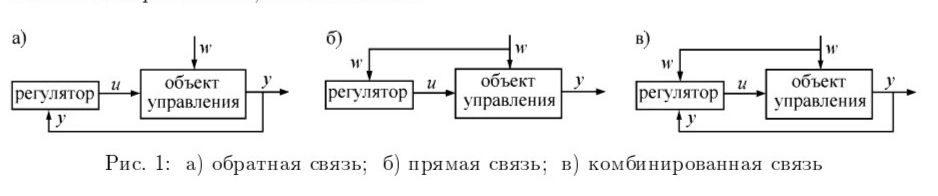
\includegraphics[width=\linewidth]{image.jpg}

%\caption{а) обратная связь; б) прямая связь; в) комбинированная связь}

\label{fig:mpr}

\end{figure}
%%%%%%%%%%%%%%%%%%%%%%%%%%%%%%%%%%%%%%%%%%%%%%%%%%%%%%%%%%%%%%%%%%%%%%%%%%%%%%%%

\section{Реализация оптимальных обратных связей в реальном времени}\label{1sec:Feedback}
Рассмотрим задачу оптимального управления
\begin{equation} \label{1problem}
    c^Tx(t_f)\to \min,
    \end{equation}
$$
    \dot{x}=A(t)x+B(t)u,\ x(t_0)=x_0^*,
    $$
$$
    x(t_f) \in X_f,\quad  u(t)\in U, \quad  t\in T,
    $$
где  $X_f=\{x\in \mathbb{R}^n: g_*\leq Hx \leq g^*\}$ --- терминальное
множество, $H\in \mathbb{R}^{m\times n}$, $g_*,$ $g^* \in \mathbb{R}^m$;
$U=\{u\in \mathbb{R}^r: u_*\le u\le u^*\}$ --- множество доступных значений
управляющего воздействия.

\begin{definition}  Управляющее воздействие $u(t)\in U$, $t\in T$, называется программой, если соответствующая ему
траектория $x(t)$, $t\in T$, математической модели (\ref{1problem}) удовлетворяет
условию $x(t_f)\in X_f$.
\end{definition}

\begin{definition}  Программа $u^0(t)$, $t\in T$,
называется оптимальной (программным решением задачи (\ref{1problem})), если на соответствующей ей (оптимальной) траектории $x^0(t)$, $t\in T$, выполняется равенство
$$
    c^Tx^0(t_f) = \min_u c^Tx(t_f),
     $$
где минимум ищется среди всех программ.
\end{definition}
%%%%%%%%%%%%%%%%%%%%%%%%%%%%%%%%%%%%%%%%%%%%%%%%%%%%%%%%%%%%%%%%%%%%%%%%%%%%%%%%

\bigskip